% Testing: the last group-project week, so it closes the arc as well as
% covering the testing chapter.
% Shared preamble for the write-on class slides.
%
% Every deck is designed to be projected and annotated live on a tablet:
% whatever takes time to draw is pre-drawn, and whatever the class produces is
% left blank. Compile a deck with `pdflatex main.tex` from its own directory,
% or run `uv run python build.py` from the repository root to build them all.
\documentclass[10pt]{article}

\usepackage[papersize={25.6cm,14.4cm}, margin=1.1cm, bottom=1.5cm,
            footskip=0.75cm]{geometry}
\usepackage[T1]{fontenc}
\usepackage[default]{sourcesanspro}
\usepackage{newtxsf}
\usepackage{tikz}
\usepackage{amsmath}
\usepackage{parskip}
\usepackage{fancyhdr}
\usetikzlibrary{arrows.meta, positioning, calc}

\setlength{\parindent}{0pt}

% Catppuccin Latte, the palette the course site uses in its light theme, so a
% deck on the projector looks like the pages the students read.
\definecolor{inkbg}{HTML}{EFF1F5}      % base
\definecolor{inksurface}{HTML}{E6E9EF} % mantle
\definecolor{inkfaint}{HTML}{CCD0DA}   % surface2, for rules and empty boxes
\definecolor{inktext}{HTML}{4C4F69}    % text
\definecolor{inkgrey}{HTML}{8C8FA1}    % overlay1, for anything secondary
\definecolor{inkblue}{HTML}{7287FD}    % lavender, the primary accent
\definecolor{inkteal}{HTML}{179299}    % teal
\definecolor{inkred}{HTML}{FE640B}     % peach, for whatever wants attention
\definecolor{inkmauve}{HTML}{8839EF}   % mauve

\pagecolor{inkbg}
\color{inktext}

% A box to write a short answer into. White against the tinted page, so it
% reads as somewhere to write rather than as part of the printed material.
\newcommand{\blank}[1][1.6]{%
  \tikz[baseline=(current bounding box.base)]{%
    \draw[inkfaint, line width=0.7pt, rounded corners=2pt, fill=white]
      (0,-0.18) rectangle (#1,0.62);}}

% A ruled area to work in. Faint dots keep handwriting level on a tablet.
\newcommand{\workspace}[2]{%
  \begin{tikzpicture}
    \draw[inkfaint, line width=0.7pt, rounded corners=3pt, fill=white]
      (0,0) rectangle (#1,#2);
    \foreach \gx in {0.5,1.0,...,#1}{%
      \foreach \gy in {0.5,1.0,...,#2}{%
        \fill[inkfaint] (\gx,\gy) circle (0.5pt);}}
  \end{tikzpicture}}

% A panel for material that is printed rather than written on.
\newcommand{\panel}[2]{%
  \begin{tikzpicture}
    \draw[inkfaint, line width=0.7pt, rounded corners=3pt, fill=inksurface]
      (0,0) rectangle (#1,#2);
  \end{tikzpicture}}

% A labelled card of printed material. #2 and #3 are widths in cm; the text
% column is the card less its padding, computed rather than guessed.
\newcommand{\cardbox}[4]{%
  \begin{tikzpicture}
    \node[draw=#1, line width=1pt, rounded corners=4pt, fill=white,
          minimum width=#2cm, minimum height=#3cm,
          text width=\dimexpr#2cm-0.9cm\relax,
          align=left, inner sep=0.45cm, text=inktext] {#4};
  \end{tikzpicture}}

% A card whose body is left blank for the class to fill in.
\newcommand{\cardblank}[4]{%
  \begin{tikzpicture}
    \node[draw=#1, line width=1pt, rounded corners=4pt, fill=white,
          minimum width=#2cm, minimum height=#3cm,
          text width=\dimexpr#2cm-0.9cm\relax,
          align=left, inner sep=0.45cm, text=inktext, anchor=north west]
      at (0,0) {#4};
  \end{tikzpicture}}

% Running header: the deck name on the left, the page's own step on the right.
% Each deck sets its name once with \deckname.
\newcommand{\deck}{}
\newcommand{\deckname}[1]{\renewcommand{\deck}{#1}}
\newcommand{\slidehead}[1]{%
  {\small\color{inkgrey}%
   \tikz[baseline=-0.5ex]{\fill[inkblue, rounded corners=1pt]
     (0,0) rectangle (0.22,0.22);}\;\deck
   \hfill \color{inkblue}\bfseries #1}\par
  {\color{inkblue}\rule{\linewidth}{1pt}}\par\vspace{0.35em}}

\pagestyle{fancy}
\fancyhf{}
\renewcommand{\headrulewidth}{0pt}
\fancyfoot[R]{\small\color{inkgrey}\thepage}

% Deck title pages, which carry no header and no page number.
\newcommand{\titleslide}[3]{%
  \thispagestyle{empty}%
  \begin{center}
    \vspace*{\fill}
    {\Huge\bfseries\color{inkblue} #1}\\[0.7em]
    {\LARGE\color{inkgrey} #2}\\[2.4em]
    #3
    \vspace*{\fill}
  \end{center}}

% One step of the plan on a title page.
\newcommand{\stepbox}[3]{%
  \node[draw=inkblue, line width=0.9pt, rounded corners=4pt, fill=white,
        minimum width=6cm, minimum height=1.7cm, align=center,
        text=inktext] (#1) at (#2,0) {#3};}

% Prompt to the room: a question the class answers, not something I read out.
\newcommand{\ask}[1]{%
  {\large\color{inkblue}\bfseries #1}\par\vspace{0.5em}}


\deckname{Testing}

\begin{document}

\titleslide{Testing}{Week 10. The last meeting week.}{%
    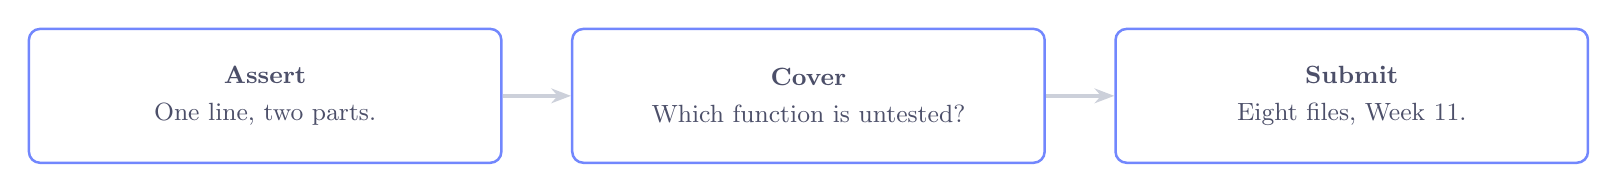
\begin{tikzpicture}[font=\small]
      \stepbox{s0}{0.0}{\textbf{Assert}\\[0.25em] One line, two parts.}
      \stepbox{s1}{6.9}{\textbf{Cover}\\[0.25em] Which function is untested?}
      \stepbox{s2}{13.8}{\textbf{Submit}\\[0.25em] Eight files, Week 11.}
      \draw[-{Stealth[length=2.5mm]}, inkfaint, line width=1.2pt] (s0) -- (s1);
      \draw[-{Stealth[length=2.5mm]}, inkfaint, line width=1.2pt] (s1) -- (s2);
    \end{tikzpicture}}

\newpage
\slidehead{You have now read all three}

\vspace{0.6cm}

\begin{center}
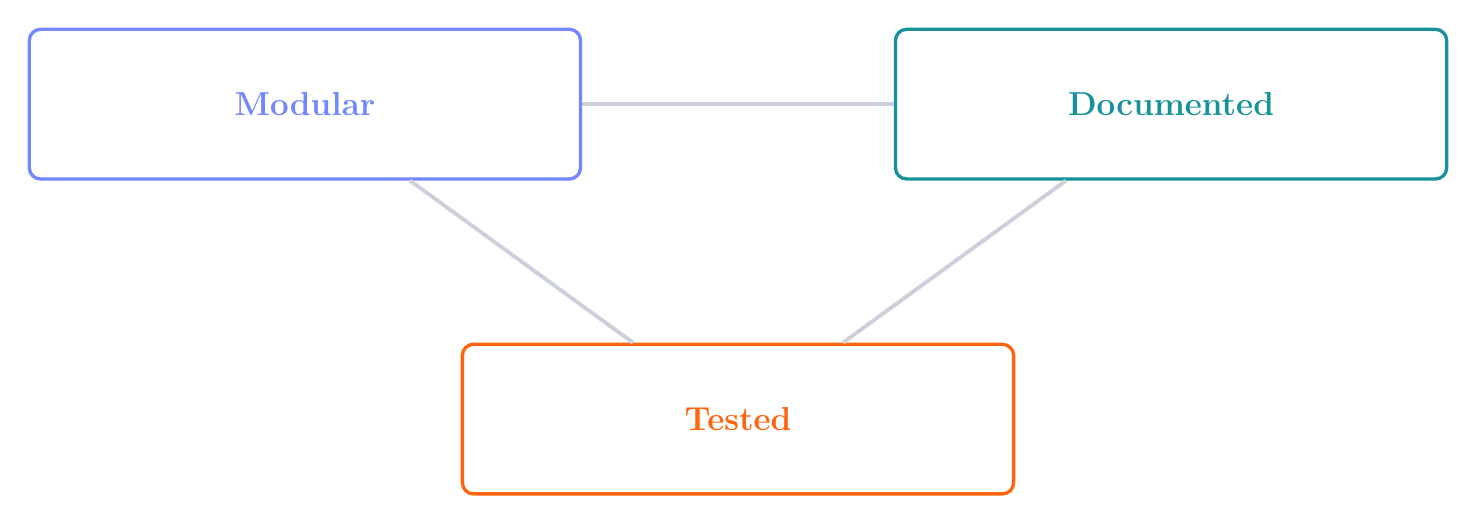
\begin{tikzpicture}
  \node[draw=inkblue, line width=1.2pt, rounded corners=4pt, fill=white,
        minimum width=7.0cm, minimum height=1.9cm, font=\large\bfseries,
        text=inkblue] (m) at (0,0) {Modular};
  \node[draw=inkteal, line width=1.2pt, rounded corners=4pt, fill=white,
        minimum width=7.0cm, minimum height=1.9cm, font=\large\bfseries,
        text=inkteal] (d) at (11.0,0) {Documented};
  \node[draw=inkred, line width=1.2pt, rounded corners=4pt, fill=white,
        minimum width=7.0cm, minimum height=1.9cm, font=\large\bfseries,
        text=inkred] (t) at (5.5,-4.0) {Tested};
  \draw[inkfaint, line width=1.4pt] (m) -- (d);
  \draw[inkfaint, line width=1.4pt] (m) -- (t);
  \draw[inkfaint, line width=1.4pt] (d) -- (t);
\end{tikzpicture}
\end{center}

\vspace{0.7cm}

\begin{center}
{\LARGE Each one makes the other two easier. Together they are
\textbf{50\%} of the project mark.}
\end{center}

\newpage
\slidehead{One line, two parts}

\vspace{1.2cm}

\begin{center}
\codebox{20.4}{assert add\_one(5) == 6, "The function gave the wrong
answer."}
\end{center}

\vspace{1.1cm}

\ask{Two things come after the word \texttt{assert}. What is each one
for?}

\vspace{0.4em}

\begin{center}
\workspace{22}{4.0}
\end{center}

\vspace{0.2cm}

{\small\color{inkgrey} A claim that must be true, and the sentence you
will read at three in the morning when it is not.}

\newpage
\slidehead{How many tests does this need?}

\vspace{0.4cm}

\begin{minipage}[t]{0.50\linewidth}
\vspace{0pt}
\codebox{11.4}{def feedback(guess, chosen):\\
\idt if guess < chosen:\\
\idt\idt return "too low"\\
\idt if guess > chosen:\\
\idt\idt return "too high"\\
\idt return "correct"}
\end{minipage}
\hfill
\begin{minipage}[t]{0.46\linewidth}
\vspace{0pt}
\ask{One test passes. Is the function tested?}

\workspace{10.6}{6.0}
\end{minipage}

\vspace{0.2cm}

{\small\color{inkgrey} Count the things the function can do, not the
number of functions. This one does three.}

\newpage
\slidehead{Your tests all pass. Are you done?}

\vspace{1.0cm}

\begin{center}

\begin{tikzpicture}
  \node at (0,0) {\cardbox{inkblue}{5.0}{2.4}{%
    {\large\bfseries\color{inkblue} Zero}}};
  \node at (5.85,0) {\cardbox{inkteal}{5.0}{2.4}{%
    {\large\bfseries\color{inkteal} One}}};
  \node at (11.7,0) {\cardbox{inkred}{5.0}{2.4}{%
    {\large\bfseries\color{inkred} Empty}}};
  \node at (17.55,0) {\cardbox{inkmauve}{5.0}{2.4}{%
    {\large\bfseries\color{inkmauve} Negative}}};
\end{tikzpicture}
\end{center}

\vspace{1.2cm}

\ask{Pick one function in your library. What does it do with each of
these?}

\vspace{1.0cm}

{\small\color{inkgrey} The top band asks for edge cases the tutorial does
not exercise. These four are where they live.}

\newpage
\slidehead{How do you test something random?}

\vspace{0.4cm}

\begin{minipage}[t]{0.48\linewidth}
\vspace{0pt}
\codebox{11.0}{import random\\[0.3em]
random.seed(0)\\
assert roll\_a\_dice() == 4\\[0.3em]
random.seed(1)\\
assert roll\_a\_dice() == 2}
\end{minipage}
\hfill
\begin{minipage}[t]{0.48\linewidth}
\vspace{0pt}
\ask{The function gives a different answer every time. So what makes this
test pass, every time?}

\workspace{11.0}{6.0}
\end{minipage}

\vspace{0.2cm}

{\small\color{inkgrey} Seeding fixes the randomness without removing it.
You can also assert the shape of a thousand rolls rather than one.}

\newpage
\slidehead{Where the tests live}

\vspace{0.4cm}

\begin{center}
\codebox{18.0}{\# test\_tsp.py\\[0.3em]
import tsp\\[0.4em]
def test\_get\_cost():\\
\idt """Check the cost of a tour we worked out by hand."""\\
\idt assert tsp.get\_cost(tour=[0, 1, 2, 0], matrix=m) == 24\\[0.4em]
test\_get\_cost()}
\end{center}

\vspace{0.8cm}

\begin{center}
{\LARGE Then, in a terminal: \quad\codebox{7.0}{python test\_tsp.py}}
\end{center}

\vspace{0.6cm}

{\small\color{inkgrey} A separate file, one function per behaviour, each
with a docstring saying what it checks. No library needed.}

\newpage
\slidehead{What is a doctest for?}

\vspace{0.4cm}

\begin{minipage}[t]{0.48\linewidth}
\vspace{0pt}
\codebox{11.0}{>{}>{}> import tsp\\
>{}>{}> tsp.get\_tour(number\_of\_stops=5)\\
{}[0, 1, 2, 3, 4, 0]}

\vspace{0.6cm}

\codebox{11.0}{python -m doctest README.md}
\end{minipage}
\hfill
\begin{minipage}[t]{0.48\linewidth}
\vspace{0pt}
\ask{You already have a test file. So why write these as well?}

\workspace{11.0}{6.4}
\end{minipage}

\vspace{0.2cm}

{\small\color{inkgrey} A doctest checks that your documentation is still
true. It is not where you test the mathematics.}

\newpage
\slidehead{So which function is untested?}

\vspace{0.5cm}

\ask{Between you, list every function in your library. Put a cross
against each one with no test.}

\vspace{0.3em}

\begin{center}
\workspace{22}{7.0}
\end{center}

\vspace{0.2cm}

{\small\color{inkgrey} This is the question to take into the meeting this
week. It turns into actions better than anything else on the agenda.}

\newpage
\slidehead{Eight files, in Week 11}

\vspace{1.0cm}

\begin{minipage}[t]{0.48\linewidth}
\vspace{0pt}
{\LARGE
\blank[0.7]\ \texttt{main.tex}

\vspace{0.8em}

\blank[0.7]\ \texttt{main.pdf}

\vspace{0.8em}

\blank[0.7]\ \texttt{references.bib}

\vspace{0.8em}

\blank[0.7]\ \texttt{<library>.py}}
\end{minipage}
\hfill
\begin{minipage}[t]{0.48\linewidth}
\vspace{0pt}
{\LARGE
\blank[0.7]\ \texttt{test\_<library>.py}

\vspace{0.8em}

\blank[0.7]\ \texttt{README.md}

\vspace{0.8em}

\blank[0.7]\ \texttt{presentation.mp4}

\vspace{0.8em}

\blank[0.7]\ \texttt{contribution.md}}
\end{minipage}

\vspace{1.0cm}

\ask{Which of the eight has your group not started?}

\newpage
\slidehead{From here to the deadline}

\vspace{0.9cm}

{\LARGE
\textbf{\color{inkblue}This week.}\quad Meet, and hand in the Week 10
minutes. That is the fifth and last.

\vspace{1.0em}

\textbf{\color{inkteal}Then.}\quad Finish the library, the tests and the
README. Write the paper. Record the presentation.

\vspace{1.0em}

\textbf{\color{inkred}Week 11.}\quad Submit the eight files, as a group.}

\vspace{1.4cm}

\begin{center}
{\large\color{inkgrey} No more timetabled meetings after this week. What
is left is yours to arrange, on your own or together.}
\end{center}

\newpage
\slidehead{Before you leave}

\vspace{0.8cm}

\begin{center}
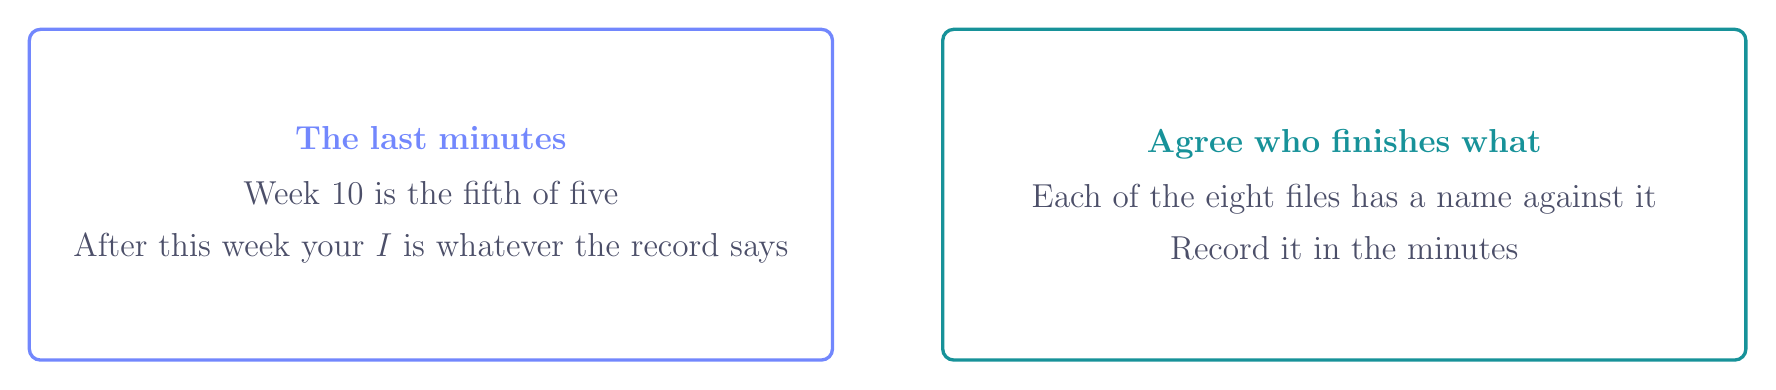
\begin{tikzpicture}
  \node[draw=inkblue, line width=1.2pt, rounded corners=4pt, fill=white,
        minimum width=10.2cm, minimum height=4.2cm, text width=9.2cm,
        align=center, inner sep=0.4cm, text=inktext, font=\large] at (0,0) {%
    \textbf{\color{inkblue} The last minutes}\\[0.5em]
    Week 10 is the fifth of five\\[0.4em]
    After this week your \(I\) is whatever the record says};
  \node[draw=inkteal, line width=1.2pt, rounded corners=4pt, fill=white,
        minimum width=10.2cm, minimum height=4.2cm, text width=9.2cm,
        align=center, inner sep=0.4cm, text=inktext, font=\large]
    at (11.6,0) {%
    \textbf{\color{inkteal} Agree who finishes what}\\[0.5em]
    Each of the eight files has a name against it\\[0.4em]
    Record it in the minutes};
\end{tikzpicture}
\end{center}

\vspace{0.9cm}

\begin{center}

\begin{tikzpicture}
  \node[draw=inkred, line width=1.4pt, rounded corners=4pt, fill=white,
        minimum width=21.8cm, minimum height=2.2cm, text width=20.6cm,
        align=center, inner sep=0.35cm, text=inktext, font=\large] {%
    \textbf{\color{inkred} Anything still unresolved comes to the contact
    hour.}\quad This is the last week it can be fixed cheaply.};
\end{tikzpicture}
\end{center}

\end{document}
